\documentclass[10pt, a4paper]{article}
\usepackage[utf8]{inputenc}
\usepackage[frenchb]{babel}
\usepackage[OT1]{fontenc}
\usepackage{amsfonts, amsmath, amssymb, amsthm, dsfont, amsthm}
\usepackage{a4wide}
\usepackage[dvipsnames]{xcolor}
\usepackage{tikz} 
\usetikzlibrary{arrows,positioning,shapes}

\title{\textbf{Lab Report} \\ Week of 12/01/2016}
%\author{Olivier \textsc{Mangin}}
%\date{\today}

\definecolor{main}{named}{BurntOrange}
\definecolor{second}{named}{RoyalBlue}
%\newcommand{\maincolor}{orange}
%\newcommand{\secondcolor}{orange!20}
\newcommand{\strong}[1]{\textcolor{main}{\textbf{#1}}}
\newcommand{\stronger}[1]{\textcolor{second}{\textbf{#1}}}
\newcommand{\colored}[1]{\textcolor{main}{#1}}

% Affichage du titre avec les numéro et date de la semaine
\newcommand{\titre}[2]{
\noindent
\hspace{-10pt}
\begin{tabular}{lr}
  \hspace{0.58\textwidth} & \hspace{0.4\textwidth} \\
  \strong{\huge Lab Report} & \textbf{\Large #1} \medskip \\
  \textbf{\Large Name \& Roll} & {\large #2} ~\\
\end{tabular}

\vspace{20pt}
}

% Encadré ``En bref'' réumant les avancées et problèmes de la semaine
\newenvironment{enbref}{
\noindent\fcolorbox{main}{main}{
\begin{minipage}{\textwidth}
\textcolor{white}{\textbf{\large }}
\end{minipage}
} \\

}{
\begin{center}
  \strong{ \rule[2mm]{\textwidth}{3pt} }
\end{center}
\vspace*{-20pt}
}

% Affichage d'un titre de rubrique
\newcommand{\rubrique}[1]{
  \bigskip
  \begin{center}
  \begin{minipage}{\textwidth}
    \noindent\strong{{\large #1} \\
      \rule[2mm]{\textwidth}{1pt} }
  \end{minipage}
  \end{center}
  \vspace*{-20pt}
}

% Symbole utilisé en début de ligne des éléments
\newcommand{\doublerect}{
\begin{tikzpicture}
  \fill[color=main] (0,0) rectangle (4pt,-4pt);
  \fill[color=second] (2pt,-2pt) rectangle (6pt,-6pt);
\end{tikzpicture}
}

% Affichage d'un titre d'élément
\newcommand{\element}[1]{
  \medskip
  \noindent\textcolor{second}{ \doublerect \textbf{#1}}
}

% Pour les lectures, petit raccourci pour mettre en avant le niveau
% de lecture d'un article.
\newcommand{\lu}{\strong{[Lu]} }
\newcommand{\parcouru}{\strong{[Parcouru]} }
\newcommand{\alire}{\strong{[A lire]} }
\newcommand{\presentation}{\strong{[Présentation]} }
\newcommand{\keynote}{\strong{[Keynote]} }



\usepackage[pdfauthor={Name}, pdftitle={Weekly}, pdfsubject={Week 1}, pdfkeywords={},colorlinks=true,urlcolor=black,linkcolor=black, citecolor=black]{hyperref}
\usepackage{listings}
\usepackage{subfig}
\usepackage{graphicx}
\lstset{%
language=Matlab,
frame=single,
%numbers=left,
%numberstyle=\footnotesize,
%tabsize=2,
keepspaces=true,
columns=fullflexible,
basicstyle=\ttfamily\scriptsize,
keywordstyle=\color{blue}
}


\begin{document}

\renewcommand{\labelitemi}{\textcolor{main}{\small $\blacktriangleright$}}
\renewcommand{\labelitemii}{\textcolor{second}{\scriptsize \textbullet}}

\titre{Week 1}{09/01/2017}

\begin{enbref}
\element{Title}
\begin{itemize}
\item Manual for OpenGL installation in Ubuntu\\
\end{itemize}
\medskip

%\element{Problèmes rencontrés}
%\begin{itemize}
%\item Néant.
%\end{itemize}
\end{enbref}

%\rubrique{Lectures}
%Néant.
%\element{\lu ... \cite{...}}

\rubrique{Installing openGL in Ubuntu}

The first step is to install the development libraries of OpenGL/Glut in Ubuntu:

\begin{itemize}
\item sudo apt-get install freeglut3 freeglut3-dev\\
\item sudo apt-get install binutils-gold\\
\end{itemize}


\rubrique{code in openGL}
\begin{lstlisting}
#include <GL/glut.h>

void init2D(float r, float g, float b)
{
	glClearColor(r,g,b,0.0);  
	glMatrixMode (GL_PROJECTION);
	gluOrtho2D (0.0, 200.0, 0.0, 150.0);
}

void display(void)
{
	glClear(GL_COLOR_BUFFER_BIT);
	glColor3f(0.0, 1.0, 1.0);

	//draw two points
	glBegin(GL_POINTS);
	for(int i = 0; i < 10; i++)
	{
		glVertex2i(10+5*i,110);
	}
	glEnd();

	//draw a line
	glBegin(GL_LINES);
		glVertex2i(10,10);
		glVertex2i(100,100);
	glEnd();

	glFlush();
}

void main(int argc,char *argv[])
{
	glutInit(&argc,argv);
	glutInitDisplayMode (GLUT_SINGLE | GLUT_RGB);
	glutInitWindowSize (500, 500);
	glutInitWindowPosition (100, 100);
	glutCreateWindow ("points and lines");
	init2D(0.0,0.0,0.0);
	glutDisplayFunc(display);
	glutMainLoop();
}
\end{lstlisting}
\begin{figure}

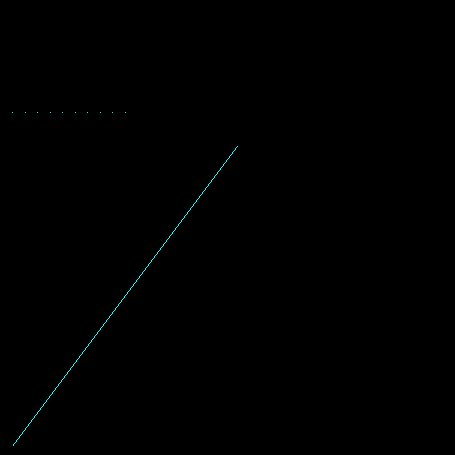
\includegraphics[scale=0.5]{abc}
\caption{example for OpenGL}
\end{figure}

\rubrique{code in matlab}
\begin{lstlisting}
y1 = sin(x.^2);
y2 = cos(x.^2);
plot(x,y1,x,y2)
\end{lstlisting}


\begin{figure}

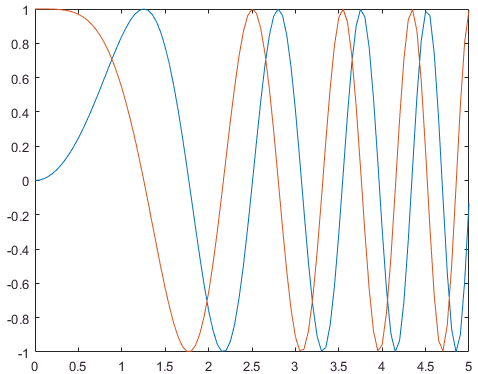
\includegraphics[scale=0.5]{def}
\caption{example for matlab}
\end{figure}



%\bibliographystyle{apalike2}
%\bibliography{../../ref}

%\begin{thebibliography}{1}

%\bibitem{Roddier}
%N.~A.~Roddier, Atmospheric wavefront simulation using Zernike polynomials, \emph{Optical Engineering} 29, 1174, 1990.

%\end{thebibliography}


\end{document}
